
\documentclass[11pt]{article}
\usepackage[utf8]{inputenc}
\setlength{\parindent}{1em}
\setlength{\parskip}{1em}
\usepackage{apacite}
\usepackage{graphicx}
\usepackage{float}
\usepackage{amsmath}
\usepackage{geometry}
\usepackage{algorithm}
\geometry{margin=4cm}
\usepackage{listings}
\usepackage{verbatim}
\lstset{language=Matlab,
        basicstyle=\ttfamily\small,
        commentstyle=\color{blue}\ttfamily\small,
        morecomment=[l]{...},
        }


\usepackage{color} %red, green, blue, yellow, cyan, magenta, black, white
\definecolor{mygreen}{RGB}{28,172,0} % color values Red, Green, Blue
\definecolor{mylilas}{RGB}{170,55,241}

\begin{document}
\title{
  Matlab prosjekt}
\author{\small Roshan Azam\\ IN3190}
\maketitle

\textbf{Oppgave1}

\begin{figure}[H]
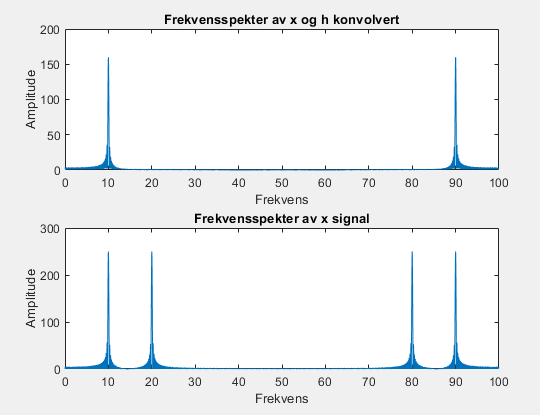
\includegraphics[scale=0.9]{1c_xh.png}
\caption{Plott av frekvensspekteret til x signalet og signalet konvolvert med filteret. Frekvens på x-aksen og amplitude på y-aksen. }
\end{figure}

\begin{figure}[H]
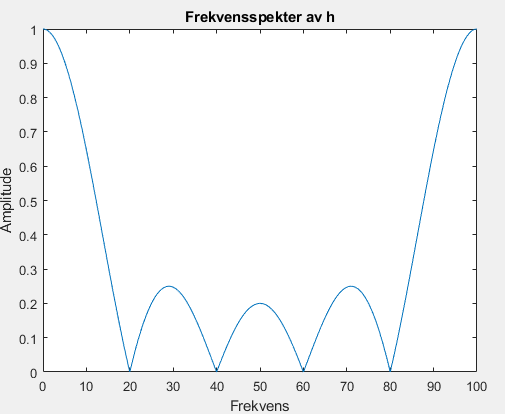
\includegraphics[scale=0.9]{1c_hfrek.png}
\caption{Plott av frekvensspekteret til filteret. Frekvens på x-aksen og amplitude på y-aksen.}
\end{figure}

Vi ser at vi får topper ved 10Hz og 90Hz på det første plott. 90Hz er bare en speiling, så vi ser bare på første halvpart av figurene for frekvensspekterene, og dette gjelder utover resten av prosjektet. Vi har to frekvenser i x-signalet, 10Hz og 20Hz. Frekvensspekteret for det konvolverte signalet har bare 10Hz, dette betyr altså at filteret har filtrert ut 20Hz fra signalet vårt, og amplituden har også blitt mindre. I frekvensspekteret til h ser vi at amplituden er 0 ved 20Hz og 40Hz, dette kan være grunnen til at det filtrerer ut 20Hz når vi konvolverer det med signalet. Uansett skal dette filteret filtrere ut de høye frekvensene.

\textbf{Kode for oppgave1:}

\textbf{Kode: konvin3190.m}
\verbatiminput{konvin3190.m}%a
 
\textbf{Kode: frekspekin319.m0}
\verbatiminput{frekspekin3190.m}%a

\textbf{Kode: oppgave1.m}
\verbatiminput{oppgave1.m}%a

\textbf{Oppgave2}
\textbf{a)}
\begin{figure}[H]
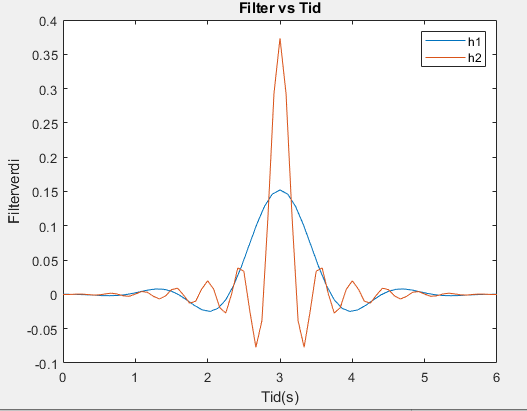
\includegraphics[scale=0.9]{2a_firtid.png}
\caption{Plott av filtrene med hensyn på tid. Filterverdi/amplitude på y aksen og tid i sekund på x aksen.}
\end{figure}

\begin{figure}[H]
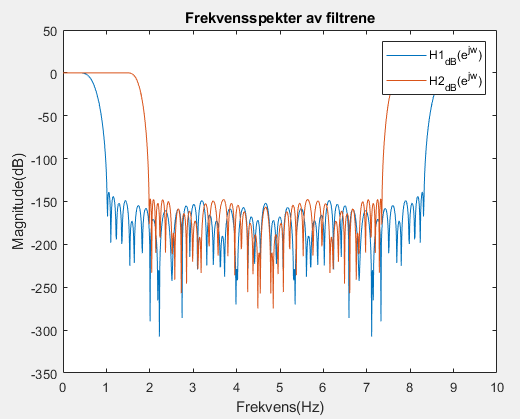
\includegraphics[scale=0.9]{2a_firfrek.png}
\caption{Plott av frekvensspekteret til de to filterene. Frekvens på x-aksen og magnitude i dB på y-aksen.}
\end{figure}

Når vi ser på frekvensspektrene til de to filtrene ser vi at de er nesten identiske. Men vi ser at h1 filtrerer lavere frekvenser enn h2, altså begynner den å filtrere før og filtrerer flere frekvenser enn h2.

\textbf{2b)}
\begin{figure}[H]
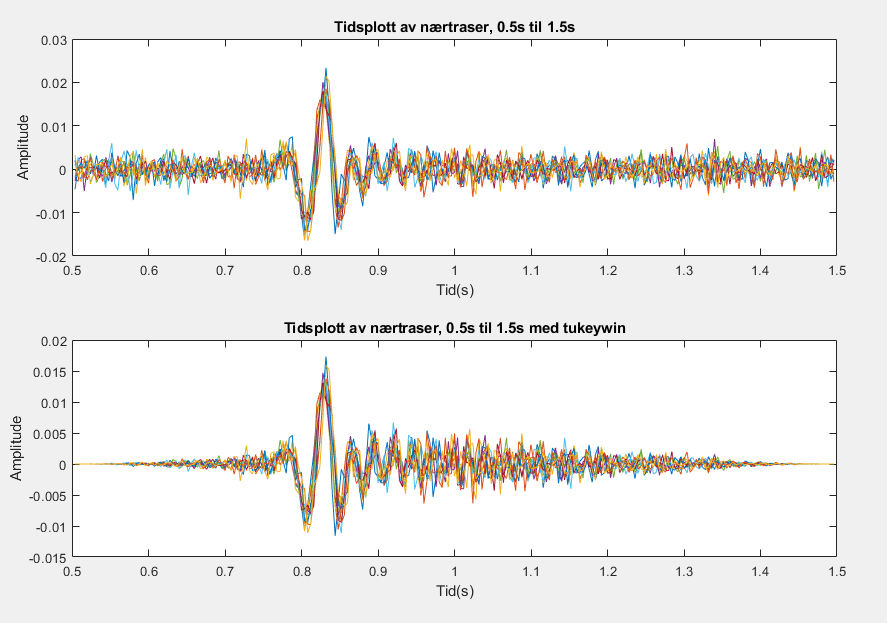
\includegraphics[scale=0.67]{2b_nertraser.png}
\caption{Plott av de 10 første trasene med hensyn på tid. Amplitude på y aksen og tid i sekunder på x aksen. Tid går fra 0.5s til 1.5s. I det nederste plottet har vi brukt Tukeywin vindusfunksjonen. }
\end{figure}


\begin{figure}[H]
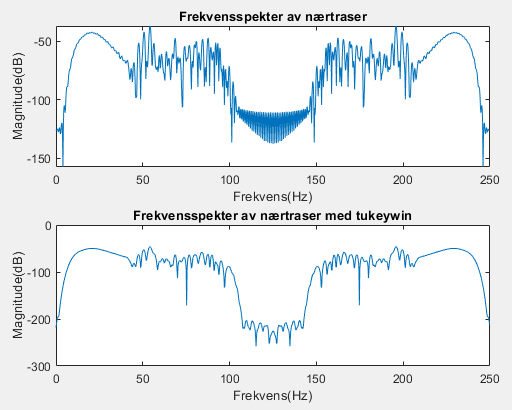
\includegraphics[scale=0.67]{2b_nertrasefrek.png}
\caption{Plott av frekvensspekteret til de 10 første trasene. Magnitude i dB på y aksen og frekvens i Hz på x aksen. I det nederste plottet har vi brukt Tukeywin funksjonen.}
\end{figure}

I denne oppgaven har vi brukt vindusfunksjonen Tukeywin(L,r). L er antall punkter, og r er hvor mye vi vil fokusere på endepunktene. Har brukt r = 1. Ser vi på frekvensspekteret vårt vil selve formen på frekvensspekteret være signalet vårt, mens de fleste utslagene vil være støy.

\textbf{2c)}

\begin{figure}[H]
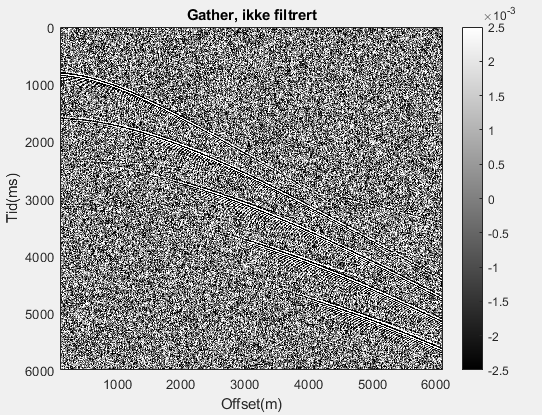
\includegraphics[scale=0.9]{2c_ufiltrert.png}
\caption{Det ufiltrerte gather plottet. Vi har offset i meter på x-aksen, og tid i ms på y-aksen.}
\end{figure}

\begin{figure}[H]
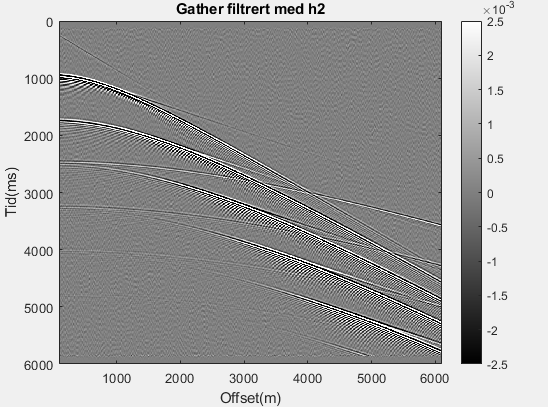
\includegraphics[scale=0.9]{2c_h2filter.png}
\caption{Gather filtrert med FIR h2. Offset i m på x-aksen, tid i ms på y-asken.}
\end{figure}

\begin{figure}[H]
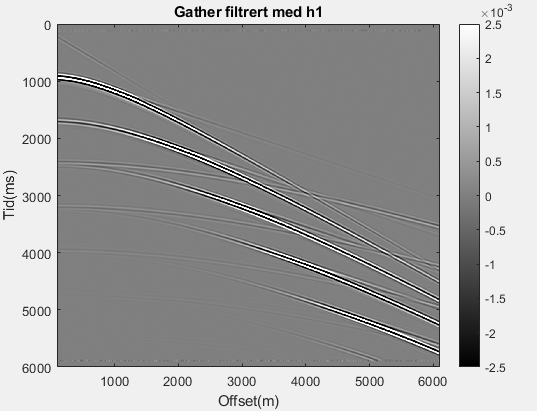
\includegraphics[scale=0.9]{2c_h1filter.png}
\caption{Gather filtrert med FIR h1. Offset i m på x-aksen og tid i ms på y-aksen.}
\end{figure}

\begin{figure}[H]
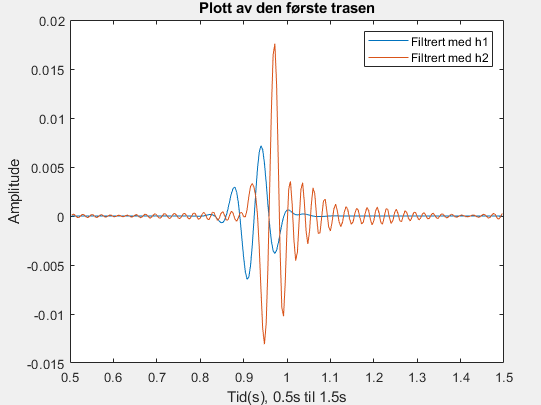
\includegraphics[scale=0.9]{2c_forstetrase.png}
\caption{Plott av første trase for begge de filtrerte gatherene. }
\end{figure}

Ser vi på figurene kan vi lett se at vi burde bruke filter 1 når vi skal filtrere gatheret vårt. I plottene med gathere er det h1 som gir mest klarhet, og i traseplottene ser vi også at signalet filtrert med h1 ikke har noe støy, men det har signalet med h2. Vi ser også fra oppgave 2a at filter h1 filtrerer flere frekvenser enn h2, så da er det naturlig at vi fortsetter å bruke h1.

\textbf{Kode for oppgave 2}

\verbatiminput{oppgave2.m}%a

\textbf{Kode for oppgave 3}
\begin{figure}[H]
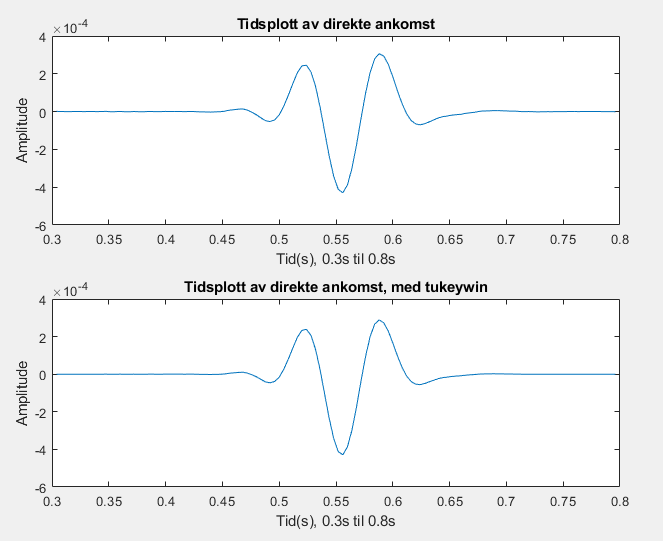
\includegraphics[scale=0.8]{3b_ankomst.png}
\caption{Plott av direkte ankomst med hensyn på tid. Tid går fra 0.3s til 0.8s, og plottet med og uten tukeywin.}
\end{figure}

\begin{figure}[H]
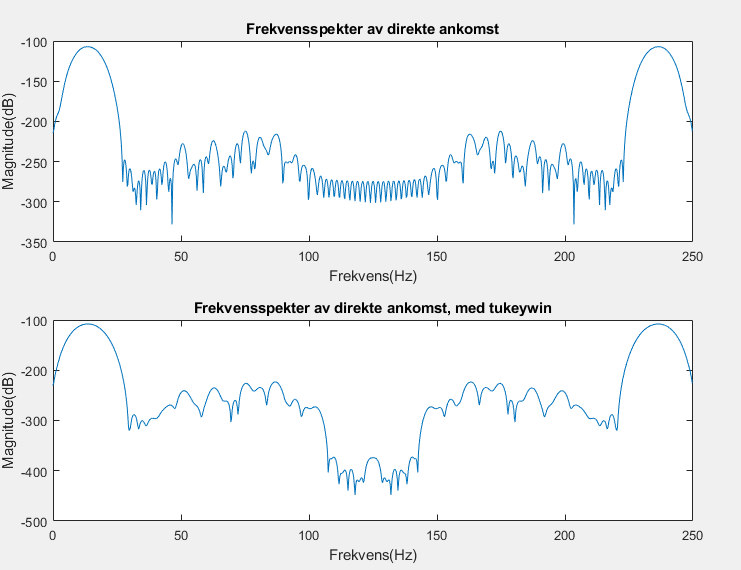
\includegraphics[scale=0.8]{3b_ankomstspek.png}
\caption{Plott av frekvensspekteret til direkte ankomst. Plottet med og uten tukeywin.}
\end{figure}

Ser vi på frekvensspekteret har vi at den dominante frekvensen er på omtrent 13.5 Hz.
Har at formel for frekvens er $f = \frac{\lambda}{c}$, der $c = 3000m/s$. Så vi har da: $\lambda = \frac{c}{f}= \frac{3000ms}{13.5Hz} = 222.22m$, vet at differansen må være omtrent 1/8 av bølgelengden for å differensiere høyden. Har da at den vertikale oppløsningen er på omtrent $222.22m*\frac{1}{8}=27.25m$

\textbf{Kode for oppgave 3}
\verbatiminput{oppgave3.m}%a

\textbf{Oppgave 4}
\begin{figure}[H]
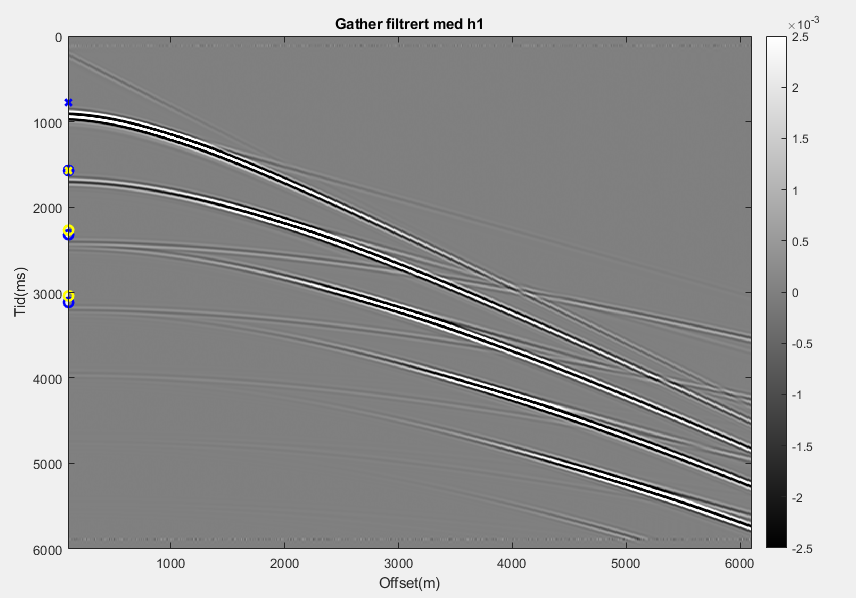
\includegraphics[scale=0.7]{4a_multippel.png}
\caption{Gatherplott med gule og blå kryss og sirkler. Offset i m på x aksen og tid i ms på y aksen.}
\end{figure}

\begin{figure}[H]
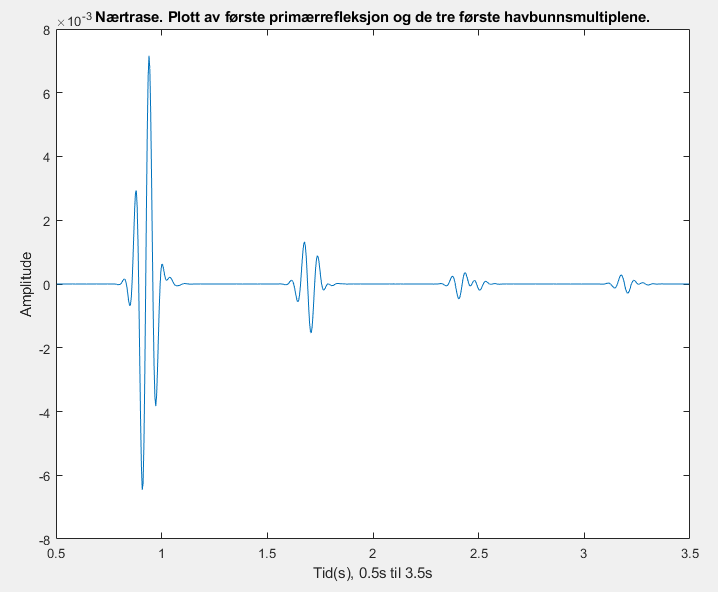
\includegraphics[scale=0.7]{4a_impuls.png}
\caption{Plott av primærrefleksjon og dens multipler i første trase. Utslag på y-aksen og tid på x-aksen.}
\end{figure}

\begin{figure}[H]
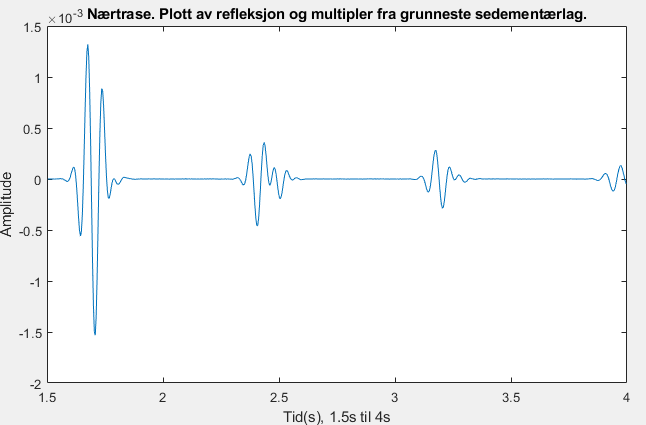
\includegraphics[scale=0.9]{4b_impuls.png}
\caption{Plott av refleksjon fra grunneste sedimentærlag. Utslag på y-aksen og tid på x-aksen.}
\end{figure}

Vi ser på plottet for første primærrefleksjon (Figur 14) og ser at tw er omkring 0.78 til 0.8s. Det blå krysset er primærrefleksjonen, de blå sirkelene er multipler, det gule krysset er refleksjon fra det grunneste sedimentærlaget og de gule sirklene er multipler av denne. 

\textbf{Kode for oppgave 4}
\verbatiminput{oppgave4.m}%a

\textbf{Oppgave 5}
\begin{figure}[H]
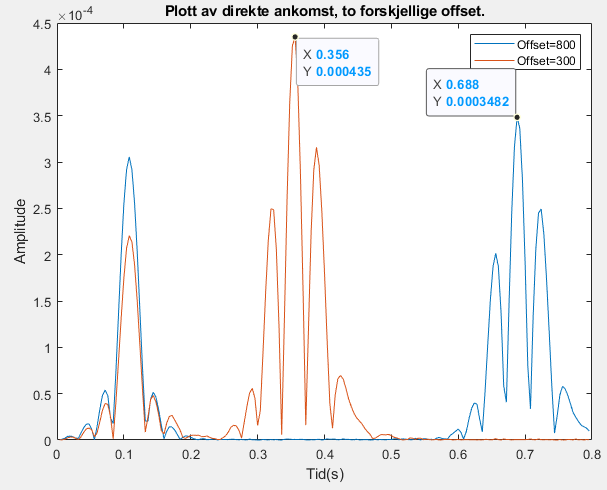
\includegraphics[scale=0.9]{5_distans.png}
\caption{Plott av direkte ankomst på to forskjellige offset, offset=800m og offset=300m. Tid i sekunder på x-akse og amplitude på y-akse.}
\end{figure}

Vi vet at $v=\frac{s}{t}$. Vi har satt offset lik 800m og 300m, så forskjellen i distanse er lik 500m. Dette er vår s. Vi kan se tid ut fra Figur 16, der vi ser på de forskjellige toppunktene til signalene. Har da $0.688s-0.356s=0.332s$. Formelen $v=\frac{s}{t}=\frac{500m}{0.332s}=1506.024m/s$, som er vårt estimat på hastigheten i vannet.

\verbatiminput{oppgave5.m}%a

\textbf{Oppgave 6}

\begin{figure}[H]
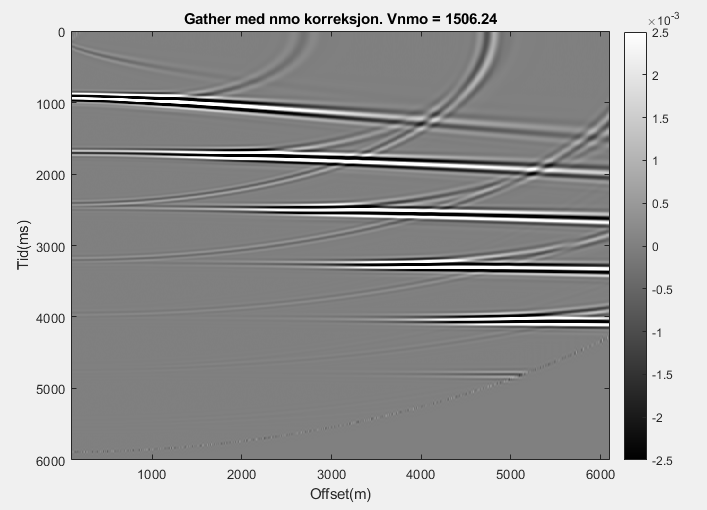
\includegraphics[scale=0.7]{6a_vnmo.png}
\caption{Plott av gather med nmo-korreksjon, der vnmo = 1506.24, som er vår estimerte hastighet av lydhastighet i vann. Offset i m på x-aksen, tid i ms på y-aksen.}
\end{figure}

\begin{figure}[H]
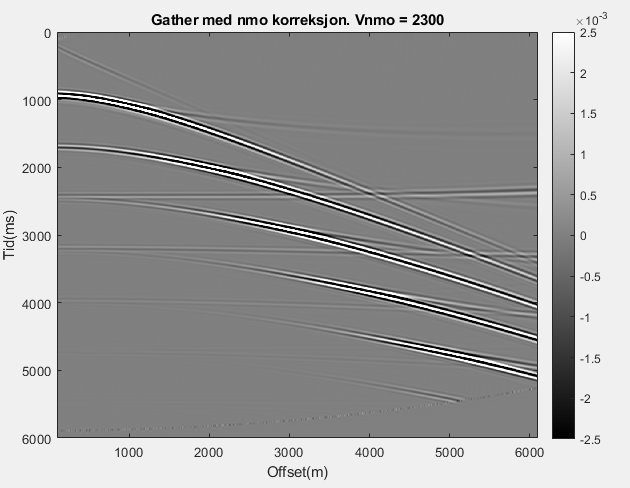
\includegraphics[scale=0.7]{6b_vnmo.png}
\caption{Plott av gather med nmo-korreksjon, der vnmo = 2300. Offset i m på x-aksen, tid i ms på y-aksen.}
\end{figure}

Jeg vil si at NMO korreksjon ikke er veldig sensitiv for forskjellige vannhastigheter. Ut fra forksjellige plott må vi ha en ganske stor forskjell i hastigheter for å få 

\end{document} 